%*******************************************************************************
%****************************** Second Chapter *********************************
%*******************************************************************************

\chapter{Data Stream Model}

\ifpdf
    \graphicspath{{Chapter2/Figs/Raster/}{Chapter2/Figs/PDF/}{Chapter2/Figs/}}
\else
    \graphicspath{{Chapter2/Figs/Vector/}{Chapter2/Figs/}}
\fi


\subsection*{Order}
The concept of \textit{Order} is rather important in Distributed system, specially Stream Processing System in particular. 

In traditional model, there are a single program, one process, one memory space running on one CPU. Programs are written to be executed in an ordered fashion like a queue:  starting from the beginning, and then going towards the end. 

In distributed system, programs are designed to solve the same problems which one can solve on a single machine using multiple interconnected machines. Although these machines are physically located across the network with possible delays or failures, the system tries to reserve the order of the result as if running on a single machine only. In other words, the ideal is that a) we run the same operations and b) that we run them in the same order - even if there are multiple machines~\citep{Mikito:2014}.

In theory, they have defined 2 types of orders: total order and partial order. 

\begin{defi}
 Paritial order~\citep{Simovici:2008} is a binary relation $\leq$ over a set $P$ which is reflexive, anti-symmetric and transitive, i.e., which satisfies for all $a$, $b$ and $c$ in $S$:
 
 \begin{itemize}
	 \item $a \leq a$ (reflexivity)
	\item  if $a \leq b$ and $b \leq a$ then $a = b$ (antisymmetry) 
	\item if $a \leq b$ and $b \leq c$ then $a \leq c$  (transitivity)
\end{itemize}
\end{defi}

A set of elements, which is partially ordered, does not always ensure the order of  2 arbitrary elements. The natural state in a distributed system is partial order. Neither in the network nor between independent nodes the system is able to make any guarantee about relative order of two elements, probably due to many factors such as network latency, performance and so on; but at each node, one can observe a local total order.

\begin{defi}
 Total order~\citep{Simovici:2008} is a binary relation `$\leq$' over a set $S$ which is anti-symmetric and transitive and total. Therefore, total order is a partial order with totality
 
 \begin{itemize}
	 \item $a \leq b$ or $b \leq a$  (totality)
\end{itemize}
\end{defi}

Total order ``<'' is strict on a set $S$ if and only if $(S, <)$ has no non-comparable pairs:
\begin{equation}
 \forall x, y \in S \Rightarrow  x < y \cup y < x 
\end{equation} 


In a totally ordered set, every two elements are comparable whereas in a partial ordered set, some pairs of elements are incomparable and hence we do not have the exact order of every element.

In streaming processing, one may not ask for entire stream  but rather a portion of data stream (i.e., window) periodically for further computation. For example, every 5 minutes, they would like to know the average volumes of last 100 transactions to detect any abnormal transaction. Any older element from $101^{th}$ will be discarded. Since the number of transactions is bounded within 100, the order of elements is crucially needed here to decide which one should fall into the window but others do not. This property also make stream processing model is different from rational data base system in which order of elements might not necessary. Traditional DBMS already knows the bounded data set involved in queries whereas stream processing engine has to decide its window based on the order.

Depend on the execution model of different systems, they may design different strategies of order such as temporal or positional order~\citep{Petit:2012}.

The \textbf{temporal order} is induced by the timestamp of elements in a stream. Using the value of timestamp, one can determine whether something happen chronologically before something else. In practice, they usually use time as a source of order. System can attach timestamps to unordered events to maintain an order between events. Nevertheless, if some elements happen simultaneously, they will have the identical timestamp, then the order is total but non-strict. For instance, there are two elements with the same timestamps but system is required to take one element only, the chosen is non-deterministic between two because there is no difference between them in term of order. Therefore, we may require a strict order in order to avoid unfortunate random choices which mislead users about data stream's insight.

The \textbf{positional order} is a strict order induced by the position of elements in stream. Two elements  may have the same timestamp but one may arrive before the other so that they have different positional orders. The positional order can be defined by arrival order or id of element regardless of an explicit timestamp. 



\subsection*{Time}
\textbf{Time Domain} $\mathbb{T}$ is a discrete, total ordered, countably infinite set of time instants $t \in \mathbb{T}$. We assume that $\mathbb{T}$ is bounded in the past, but not necessarily in the future.

Time instant can be signified by either human-readable formatted string  such as ``Wed Aug 21 2013 00:00:00 GMT-0700 (PDT)'' or a \textit{Long} number as a milliseconds time value. In many high-level languages, the ``zero epoch'' moment $t = 0$ is usually set to the midnight of \textit{Jan 1 1970} and time unit is millisecond. Obviously, it is exchangeable between 2 representing formats.   
For the sake of simplicity, we will assume that the time domain is the domain of non-negative long number ($\mathbb{T} = \mathbb{N}$) {0,1,2,3,..} and totally ordered~\citep{Dindar:2013}.

When considering the order, each event may be attached with either or both of : system time $t_{sys}$ (implicit) and application time $t_{app}$ (explicit). 

\textbf{Application Timestamps $t_{app}$}. In many case, each element in stream contains an explicit source-assigned timestamp itself. In other words, the timestamp attribute may be a part of the stream schema. To consider  a common log format for a web application which contains a timestamp specifying when the action is taken place. 
A log line records an action of user \textit{pablo} to get an image on Oct 10 2000:
\begin{verbatim}
216.58.209.174 user-identifier pablo [10/Oct/2000:13:55:36 -0700] 
"GET /image.gif HTTP/1.0" 200 1234
\end{verbatim}
Since web server may handle thousands of concurrent requests per second, it is possible to have many line of logs sharing a $t_{app}$ timestamp value. Therefore, application timestamp can be used as a source of total but non-strict ordering.

\textbf{System Timestamps $t_{sys}$}. Even if the element arrives at the system are not equipped with a timestamp, the system assigns a timestamp to each tuple, by default using the system’s local clock. While this process generates a raw stream with system timestamps that can be processed like a regular raw stream with application timestamps, one should be aware that application time and system time are not necessarily synchronized~\citep{Kramer:2009}. Since system timestamp is assigned implicitly by system, one may not notice its presence on schema. 


Both application and system timestamp captures time information but they carry two different meanings. The former is related to the occurrence of the application event (when the event happens), whereas the latter is related to the occurrence of related system (when the corresponding event data arrive at system). Multiple elements may have the same application timestamps but they will not arrive in the same order. Therefore, system will assign the different unique system timestamp based on their arrival. System then can believe in the system timestamp as a strict total ordered basis for reasoning about arrival elements to perform processing. For example, another log from different users arrive at system:
\begin{verbatim}
219.53.210.143 user-identifier fabio [10/Oct/2000:13:55:36 -0700] 
"GET /image.gif HTTP/1.0" 200 1432
\end{verbatim}
However, it might arrive after the first log for user \textit{pablo} then system would response \textit{pablo}'s first, instead of \textit{fabio}'s request.

As we mentions above, in general, time domain is total ordered in local machine, but partial ordered across the system because of possible postponements on processing or asynchronous timestamp at different nodes. From now on, we are going to analyze the execution model of stream processing on logical layer which means that it work like it would on a single machine. Thus, we could assume that time domain is the source for total ordering.

%\textbf{\\TODO}: more on Timestamp in Streams~\citep{Babcock:2002} page 13

\subsection*{Tuple}
A tuple is a finite sequence of atomic values. Each tuple can be defined by a \textit{Schema} corresponding to a composite type. Tuple can represent a relational tuple, a event or a record of sensor data and so on~\citep{Arasu:2006}. For instance, the line of log in the previous example follows a schema:

\begin{verbatim}
<SourceIP, IdentityType, user, timestamp, action, response, packageSize>
\end{verbatim}

A data tuple is the fundamental, or atomic data element, embedded in a data stream and processed by an application. A tuple is similar to a database row in that it has a set of named and typed attributes. Each instance of an attribute is associated with a value~\citep{Henrique:2014}. Furthermore, one can consider a tuple as a partial order mapping a finite subset of attribute names to atomic values~\citep{Petit:2012}. A tuple consists of a set of \textit{(Attribute $\times$ Value)} pairs such as $(SourceIP,\,219.53.210.143)$


\section{Stream Model}


Based on time and tuple domain, basically, CQL language in STREAM engine~\citep{Arasu:2006} defines a data stream as
\begin{defi}
	A stream $\mathbb{S}$ is a countably continuous and infinite set of elements $s:<v,t> \in \mathbb{S}$, where $v$ is a tuple belonging to the schema of $\mathbb{S}$ and $t \in \mathbb{T}$ is the timestamp of the element. 
\end{defi}

There are several definitions of data stream varying based on the execution model of systems. On the previous definition, a timestamp attribute can be a non-strict total ordered application timestamp so that system may not rely on it to select tuples on some operations requiring proper order between any pair of tuples. For this reason, stream can contain an extra physical identifier  $\varphi$~\citep{Petit:2010} such as increment tuple id to specify its order. The tuple with smaller id mean that they arrive and should be processed before the tuples with bigger id. Another way to identify the order of a tuple element is to separate the concept of application and system timestamp. In SECRET model~\citep{Dindar:2013}, each stream element is composed of a tuple for event contents, an application timestamp, a system timestamp, and a batch-id value. The idea of batch-id is critical to SECRET system we do not mention in the thesis.
In short, we learn that elements of a stream are totally strict-ordered by the system timestamp and physical identifier.

In Apache Flink, for the flexibility, system accepts a user-defined timestamp function   $f: \mathbb{TP} \rightarrow \mathbb{T}$ to map a tuple to its application timestamp value. One of the most common scenario is that the function $f$ extracts one attribute of Schema and consider it as timestamp value.

Consider the example of temperature sensors, the sensors feed a stream $s(TIME\ :\ long,TEMP:\ int)$ indicating that at the moment of \textit{TIME}, the ambient temperature is \textit{TEMP}. Since $TIME$ attribute has the $long$ data type, we are able to consider it as a timestamp value due to function
\begin{equation}
f: s(TIME, TEMP) \rightarrow TIME
\end{equation}

However, we may receive the stream signal from a different timezone. Thus, the application timestamp must be converted to the current timezone for the sake of data integration. For instance, one acquires the timestamp value (in seconds) in next timezone.
\begin{equation}
f: s(TIME, TEMP) \rightarrow TIME + 3600
\end{equation}

%%I propose the definition of Stream $s:<v>$ extends to $s:<v, t_{app}, t_{sys}>$, with $t_{app} = f(v)$, $t_{app} \in \mathbb{T}$, $t_{sys} \in \mathbb{T}$

For further analysis on execution model in Apache Flink, I propose a extend definition of a data stream as:

// TODO: Zoltan: Why this definition is "good", interesting, important, usefull for us? 

\begin{defi}
	A stream $\mathbb{S}$ is a countably infinite set of elements $s \in \mathbb{S}$. Each  stream element $s: <v, t_{app}, t_{sys}>$, consists of a relational tuple v conforming to a schema $S$, with an \textit{optional} application time value $t_{app} \in \mathbb{T}^*$ with $\mathbb{T}^* = \{-1\} \bigcup \mathbb{T}$ and a timestamp $t_{sys} \in \mathbb{T}$ generated automatically by system, due to the event arrival.
\end{defi}

With the partial function $f$ to extract an application timestamp value from tuple: $f: \mathbb{TP} \rightarrow \mathbb{T}^*$ with tuple domain $\mathbb{TP}$, time domain $\mathbb{T}^*$
\begin{equation}
	t_{app} = 
	\begin{cases}
		f(v) \qquad\qquad \textsl{ if function}\, f\, \textsl{is  defined}\\
		   \\
		-1 \qquad\qquad\qquad \textsl{ otherwise}
	\end{cases}
\end{equation}



 
\subsection*{Data Stream Properties} 
In the data stream model, some of all the input data that are to be operated are not available for random access from disk or memory, but rather arrive as one or more continuous data streams. 

%Data streams differ from the conventional stored relation model in several ways~\citep{Babcock:2002}

Data Stream may have the following properties~\citep{Golab:2010}:
\begin{itemize}
	\item They are considered as sequences of records, ordered by arrival time or by another ordered attributed such as generation time which is explicitly specified in schema, that arrive for processing over time instead of being available a priorie.
	
	\item They are emitted by a variety of external sources. Therefore, the system has no control over the arrival order or data rate, either within a stream or across multiple streams.
	
	// TODO: Zoltan: yes but some considerations should be made not?
What if the "almost" totality of the data arrives in reverse time order? how to buffer? how to process too fast data rate?
what does it means too fast?
etc...

	\item They are produced continually and, therefore, have unbounded, or at least unknown, length. Thus, a DSMS may not know if or when the stream ``ends''. We may set a time-out waiting for new event. Exceeding the time-out, the stream considerably terminated. 
	
	\item Typically, big volume of data arrives at very high speed so that data need to process on the fly. Once an element from a data stream model has been processed it is discarded or archived. Stream elements cannot be retrieved, unless it is explicitly stored in storage or memory, which typically is small relative to the size of the data stream~\citep{Babcock:2002}.
	
\end{itemize}


\subsection*{Stream Representations}
\subsubsection*{Base Stream vs. Derived Stream}
They distinguish 2 kinds of streams~\citep{Kramer:2009} \textit{base stream}(source stream) and \textit{derived stream}. Base stream stream is produced by the sources whereas derived stream is produced by continuous queries and their operators~\citep{Arasu:2006}. 
%For example,~\citep{Golab:2010} page 17
From now on, we give example queries on input stream named \textit{StockTick}~\citep{StreamBaseTut} and the schema associated with the incoming tuples includes 4 fields:
\begin{itemize}
\item \textbf{Symbol}, a string field of maximum length 25 characters that contains the symbol for a stock being traded (e.g. IBM);
\item \textbf{SourceTimestamp}, a timestamp field containing the time at which the tuple was generated by the source application(timestamp is represented with date time format or long integer);
\item \textbf{Price}, a double field containing transaction price
\item \textbf{Quantity}, a integer fields that contains the transaction volume
\item \textbf{Exchange}, a string field of maximum length 4 that contains the name of Exchange the trade occurred on (e.g. NYSE)

\end{itemize}
A sample tuple represents the price of IBM stock unit is 81.37 at ``1 May 2015 10:18:23" from NYSE market. And 30.000 units is sold in the transaction. 
\begin{verbatim}
<IBM,1430468303,81.37,30000,NYSE>
\end{verbatim}

The \textit{StockTick} is emitted directly from a source so that it is a base stream. However, a below \textit{HighStockTick} stream is a derived stream originated from \textit{StockTick}. \textit{HighStockTick} contains only transaction of stocks with price of more than \$100 per unit.

\begin{verbatim}
CREATE STREAM HighStockTick AS
	SELECT * FROM StockTick 
	WHERE price > 100
\end{verbatim}

In practice, base stream are almost always append-only, mean that previously arrived stream elements are never modified. However, derived stream may or may not be append-only\cite{Golab:2010}. A derived stream that present the average transaction volumes between interval time $[t_1, t_2]$. The query produce an element $s_1$ to the stream immediately after $t_2$. However, an element of \textit{StockTick} stream with timestamp 
$t_{12} \in [t_1,t_2]$ arrive late at $t_2+\phi$. If the system takes into account of the late arrival element, it will update the previous average volumes at $[t_1, t_2]$. In this case, this derived stream is not append-only. Unfortunately, Flink has not supported Delay function by this time, so that all streams are append-only.


%\textbf{Note}: another examples from \textbf{epl-guide}
%\textbf{Note}: stock example : http://www.codeproject.com/Articles/553206/An-Introduction-to-Real-Time-Stock-Market-Data-Pro


\subsubsection*{Logical Stream vs. Physical Stream}
%// TODO : Logical vs. physical stream ? ~\citep{Kramer:2009}

Logical stream is a conceptual and abstract data stream which is processed linearly through a series of chaining operators. According to logical data flow graph, one is able to observe the order of operators that data is processed and what are the input and output of process.

Physical stream flow graph indicates how system really process the data in parallelism environment. Physical operator is replicated and the internal operator state is partitioned and segmented. Figure~\ref{fig:streamRepresent} depicts the different between logical and physical data flow.
A logical stream from source go straight through an aggregate and a filter operator before written to Sink, whereas physical streams are segmented and go through different internal replica of the same logical operator. Eventually, all physical streams will be merged and written to one Sink. 

%\begin{wrapfigure}{l}{0.7\textwidth} 
 %   \centering
  %  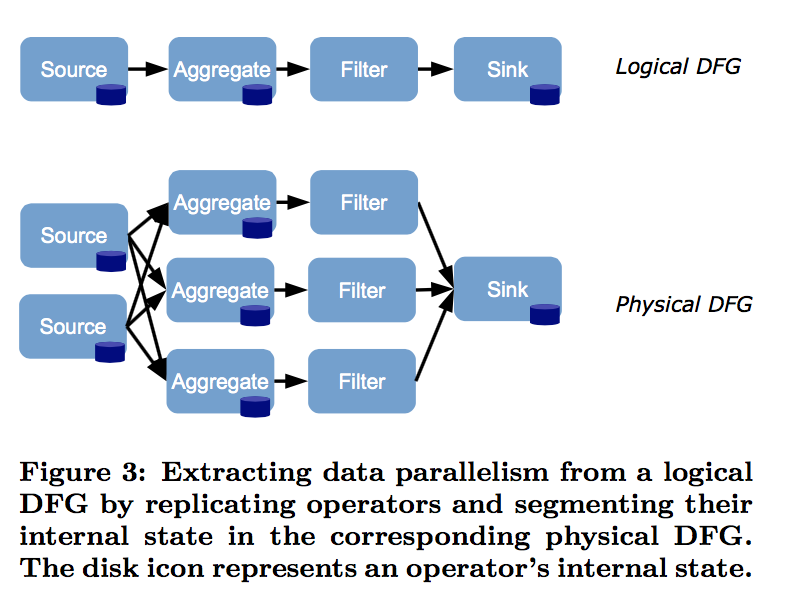
\includegraphics[width=0.7\textwidth]{logicalPhysicalDataFlow}
%\caption[Minion]{Stream Processing in Action. Henrique Andrade}
%\label{fig:streamRepresent}
%\end{wrapfigure}

\begin{figure}[htbp!] 
\centering    
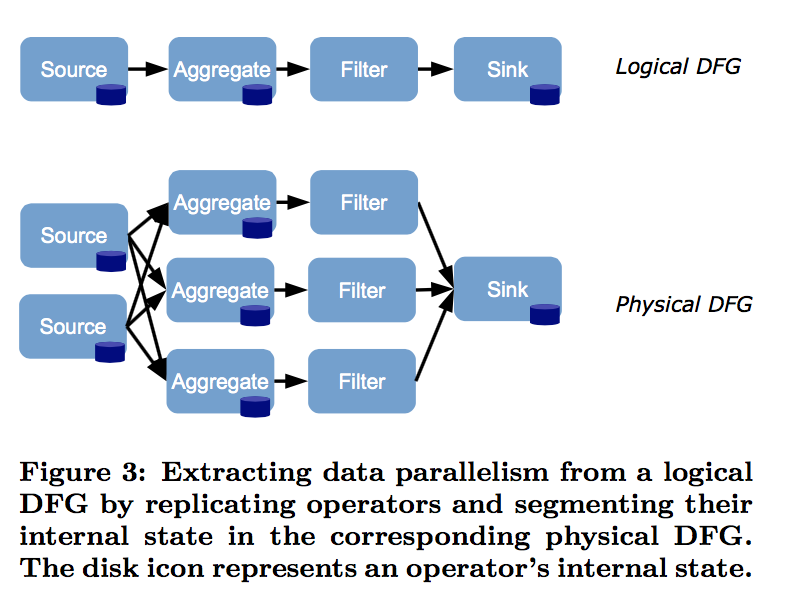
\includegraphics[width=0.7\textwidth]{logicalPhysicalDataFlow}
\caption[Logical and Physical Stream]{Extract data parallelism from a logical Data Flow Graph(DFG) by replicating operators and segmenting their internal state in the corresponding physical DFG. The disk icon represent an operator's internal state~\citep{Henrique:2013}}
\label{fig:streamRepresent}
\end{figure}

   
%\subsection*{Signals[Option]~\citep{Golab:2010}}     
    
    
\section{Stream Windows}

From the system's point of view, it is often infeasible to maintain the entire history of the input data stream. Because data stream is running infinitely, we may not know exactly when it ends. It nearly impossible to query over the entire stream with some operators such as sum, average. Accumulating a tuple attribute for entire stream may results to a very big value causing  buffer overflow.  When a bounded amount of memory is limited, hence it is barely capable of producing exact answers for data stream queries. Nevertheless, high-quality approximate answers are often acceptable instead. 

We have seen many techniques to tackle the problem such as sketches, random sampling, histogram and so on. However, the most preferred is \textit{windowing technique} which continually runs queries over recent portion of data stream  in lieu of then entire of its past history. For examples, every 10 minutes, asking for total numbers of transaction happened last hour only. The semantic of window is clear and well-defined that makes it easy to operated by system and understood by users. The size of window is relatively smaller than size of stream so that system can keep latency of computation low.  More importantly, from the user's point of view, recent data may be more insightful and informative to make a data-driven decision immediately. Those reasons motivated the use of windows to restrict to the scope of continuous queries. Indeed, many stateful stream processing operators are designed to work on windows of tuples, making it a fundamental concept in stream processing. Therefore, a stream processing language must have rich windowing semantics to support the large diversity in how stream processing engine can consume data on a continuous basis.


\begin{defi}
A \textbf{Window} $W$ \cite{Dindar:2013} over a stream $\mathbb{S}$ is a finite subset of stream $\mathbb{S}$ 
\end{defi}


A window over streaming data can be created, buffering a continuous sequence of individual tuples. However, the size of window is a finite number so that system must decide what and how to buffer data based on the window specification. 

The specification consists of several parameters :
\begin{enumerate}
\item An optional \textbf{partitioning clause}, which partitions data in window into several groups. Query on window will be taken place regard for each group, instead of the whole window
\item A window \textbf{size}, that may be expressed either as the number of tuples included in it or as the temporal interval spanning its contents
\item A window \textbf{slide}, the distance between the starts of 2 consecutive window (i.e., waiting 2 seconds or 5 data elements before starting a new window). This crucial property determine whether and in what way a window change state over time. If the window slide parameter is missing, system can  assign implicitly that the slide size is equal to the window size. In this case, we have a stream of disjoint windows so called batch windows or tumbling windows.
\item An optional \textbf{filtering predicate}, keeping only elements that satisfy the predicate.
\end{enumerate}

For example, a window specification:
\begin{lstlisting}
	[
		SIZE 3 hours EVERY 1 hours 
	 	PARTITIONED BY Exchange
	 	WHERE Quantity > 100.000
	 ]
\end{lstlisting}
means that window cover all transactions with $Quantity > 100.000$ over last 3 hours once every 1 hour. Transaction tuples inside the window are partitioned into groups specified by Exchange keyword (Figure~\ref{fig:winSpec})

\begin{figure}[htbp!] 
\centering    
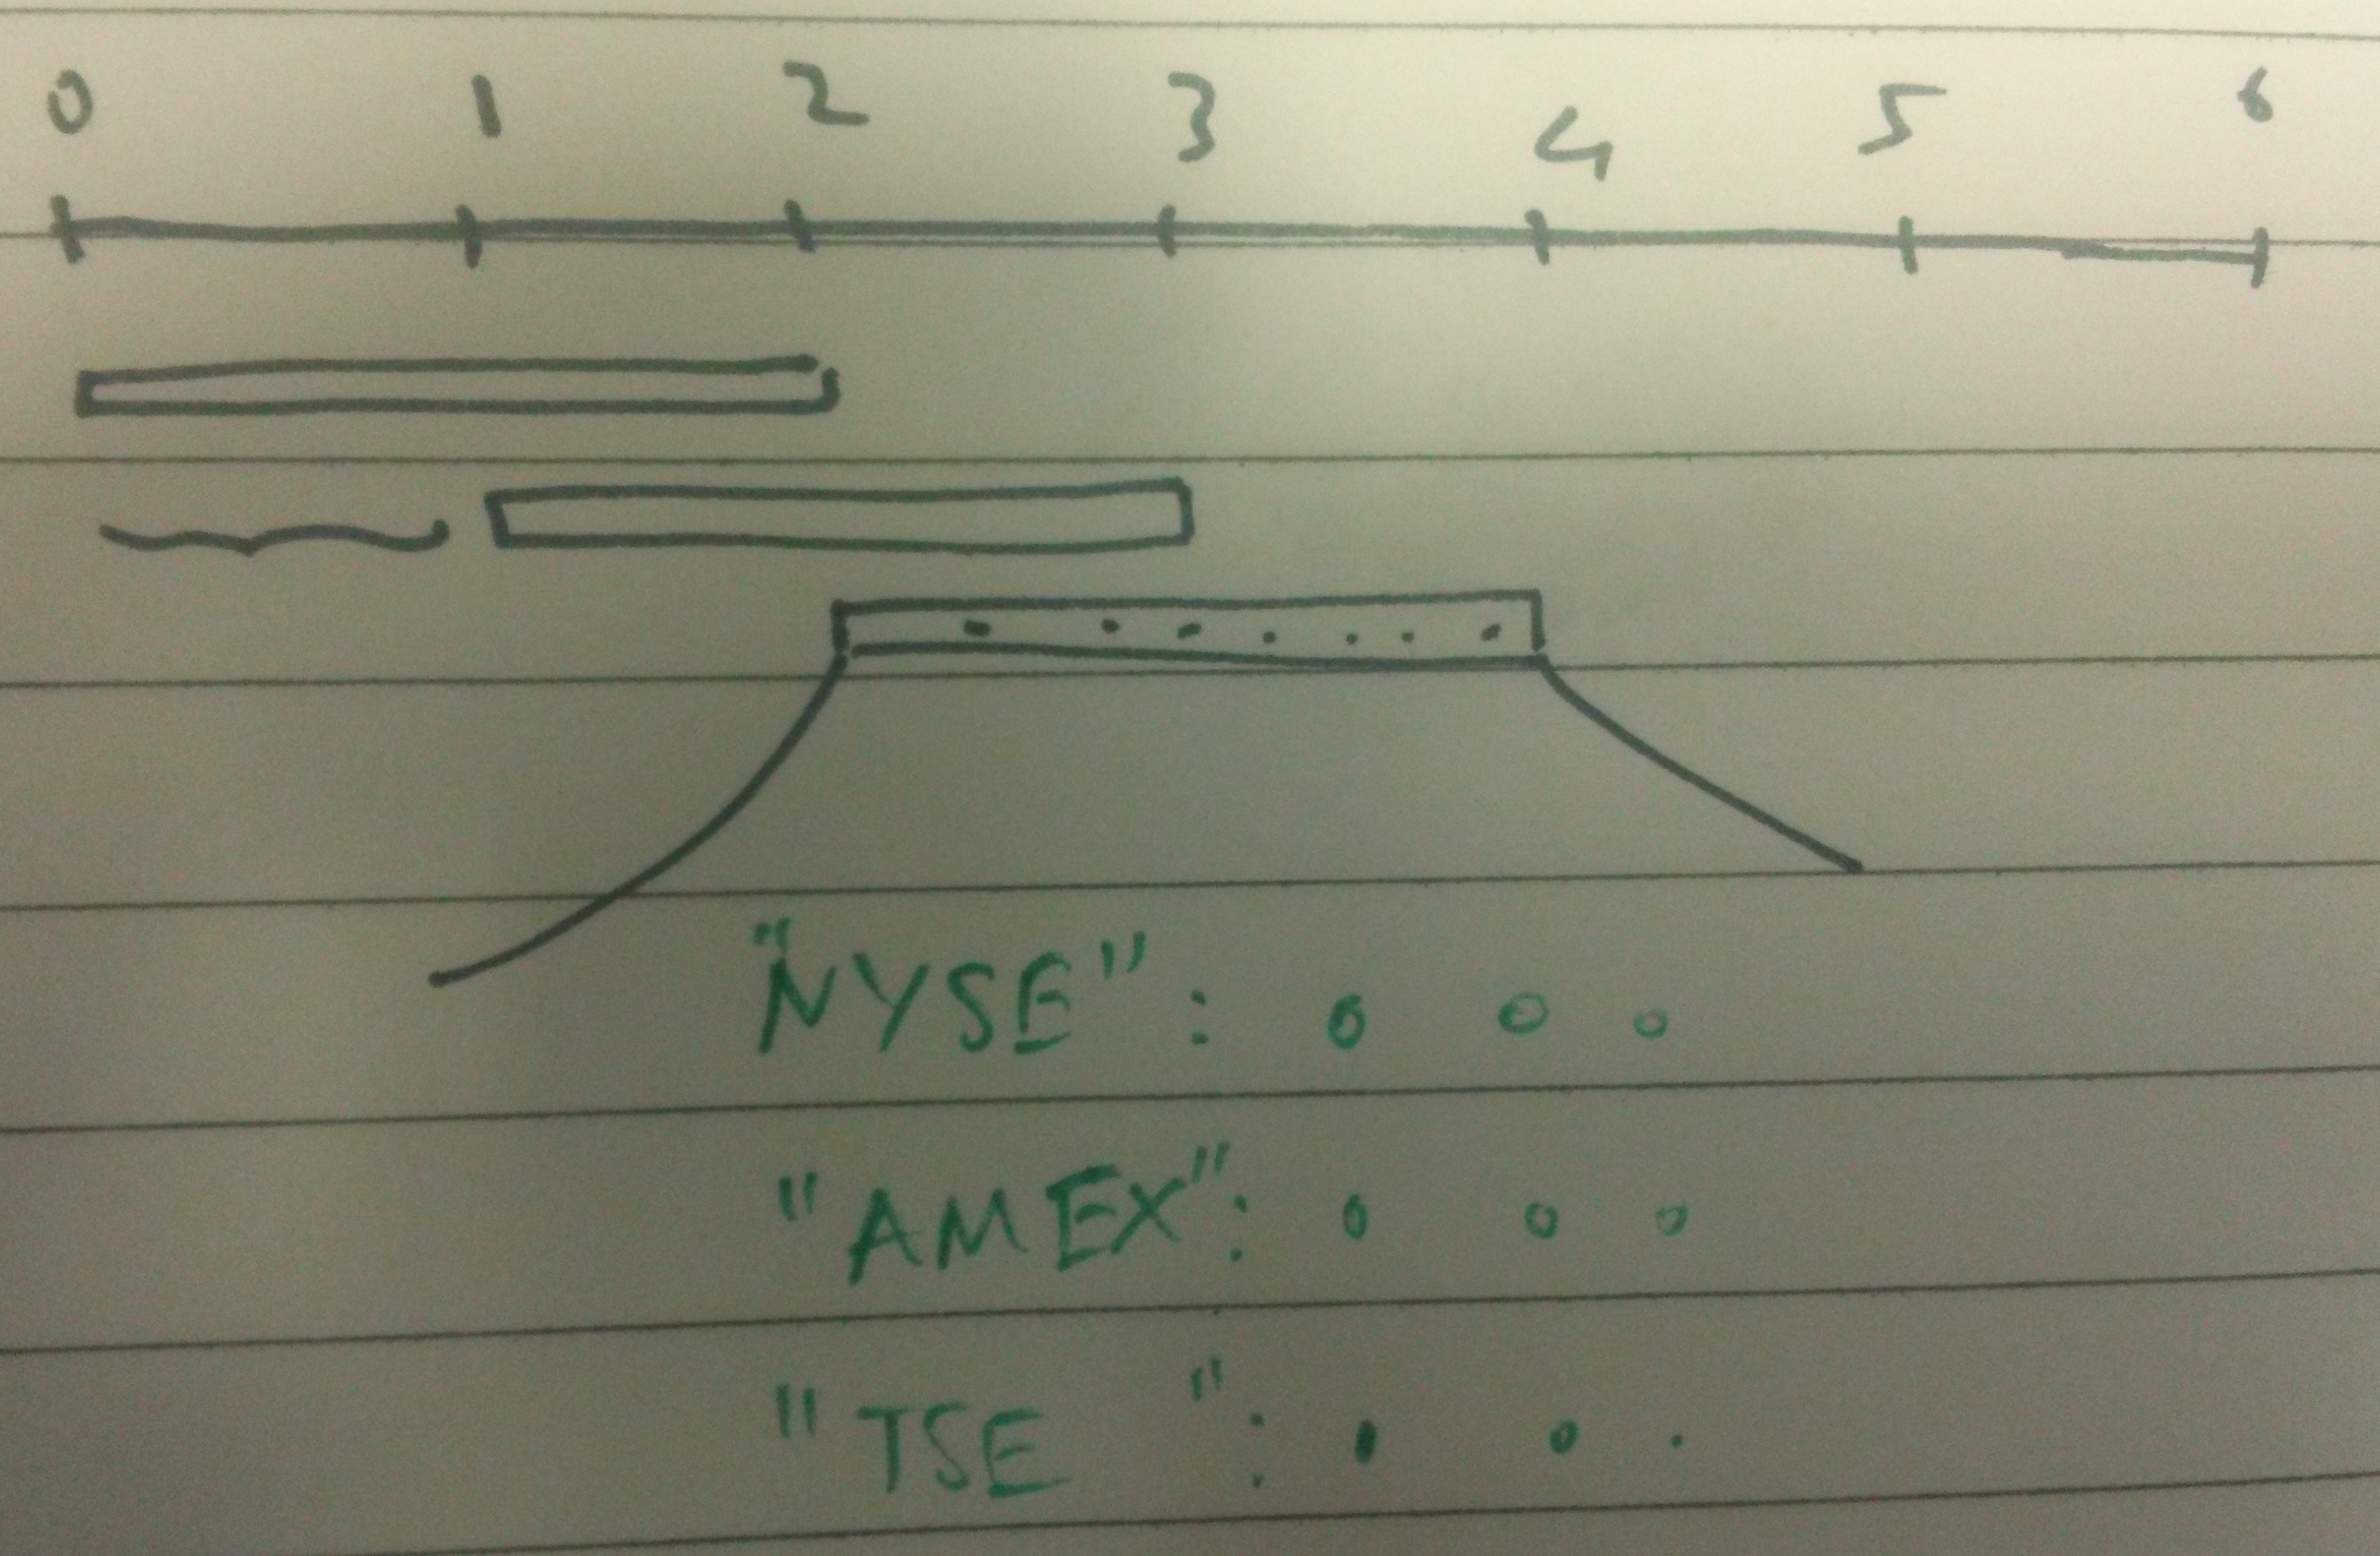
\includegraphics[width=0.7\textwidth]{winSpec}
\caption[Windowed Stream]{Windowed Stream (i.e., Stream of Windows)}
\label{fig:winSpec}
\end{figure}

In the example, we obtain 2 windows based on window size, window slide and predicate condition: 
\begin{itemize}
	\item Window 1 : $W_1:\{S_1,\,S_2,\,S_3,\,S_4,\,S_5,\,S_6\}$
	\item Window 2 : $W_1:\{S_2,\,S_3,\,S_4,\,S_5,\,S_6,\,S_7\}$
\end{itemize}
However, inside each window, system divides tuples into groups by Exchange keywords. For examples, in window $W_2$, there are 3 groups of tuples: ``NYSE'':$\{S_2,\,S_3,\,S_4\}$, ``AMEX'':$\{S_3,\,S_7\}$, ``NYSE'':$\{S_6\}$. Aggregation operators such as count, sum, average will be applied to each group. In case the partitioning clause is undefined, those operators will be executed on the whole window $W_1$, $W_2$ instead.
 
Windows can be constructed according to \textit{window specification} that defines what to buffer, resulting in many window variations. These variations differ in their policies with respect to evicting old data that should no longer be buffered, as well as in when to apply query operators on window buffer. Window may be classified according the following criteria:

\subsection{Direction of movements}
Window can fixed or sliding along the stream.
\begin{itemize}

\item \textbf{Fixed Window}:  has both upper-bound and lower-bound fixed. Therefore the window is evaluated only once and captures a constant portion information of stream. For instance, window stores the transactions generated in 2 hours from ''2015/01/01 12:00:00" to ''2015/01/01 14:00:00"

\item \textbf{Landmark Window}: One of the bounds remains  anchored at a specific system timestamp. The other edge of the window is allowed to move freely. Usually, the lower-bound is fixed, and the upper-bound shifted forward in pace with time progression.
For example, windows capture all transaction from 1 a.m once every hour (Figure~\ref{fig:landMarkWin}).

\begin{figure}[htbp!] 
\centering    
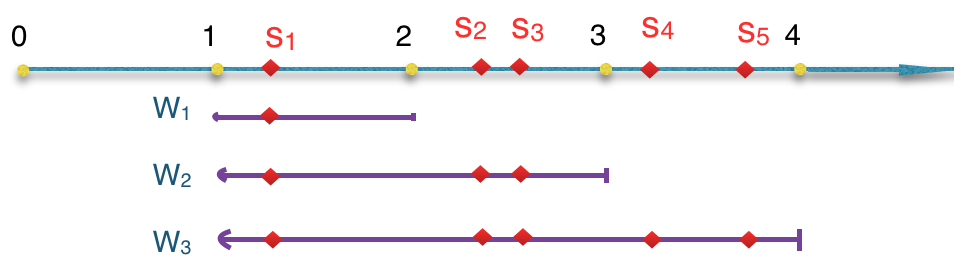
\includegraphics[width=0.7\textwidth]{landMarkWin}
\caption{Landmark Window}
\label{fig:landMarkWin}
\end{figure}

Up to 4 a.m, the stream contains 3 windows: 
\begin{itemize}
\item $W_1(1,2):\{s_1\}$ 
\item $W_2(1,3):\{s_1, s_2, s_3\}$ 
\item $W_3(1,4):\{s_1, s_2, s_3, s_4,s_5\}$ 
\end{itemize}

\item \textbf{Sliding window}: the width of the window may be fixed in term of logical unit (i.e., time interval unit) or physical unit (i.e., tuple count in window). However, the boundaries of windows change overtime along the stream.

For example, window contains last 3 transactions once every 1 transaction passed. Up to 4am, the stream contains 5 windows. Figure~\ref{fig:slideWin}
\begin{itemize}
\item $W_1:\{s_1\}$ : at the beginning there is only tuple $s_1$ on stream
\item $W_2:\{s_1, s_2\}$ there are only tuple $s_1$ and $s_2$ on stream. Window may take up to 3 tuples so that both $s_1$ and $s_2$ are included  
\item $W_3:\{s_1, s_2, s_3\}$ 
\item $W_4:\{s_2, s_3, s_4\}$ there are 4 tuples on stream but window can take last 3 tuples only. Therefore, window buffer will insert $s_4$ and drop $s_1$
\item $W_5:\{s_3, s_4,s_5\}$  window buffer insert $s_5$ and drop $s_2$
\end{itemize}

\begin{figure}[htbp!] 
\centering    
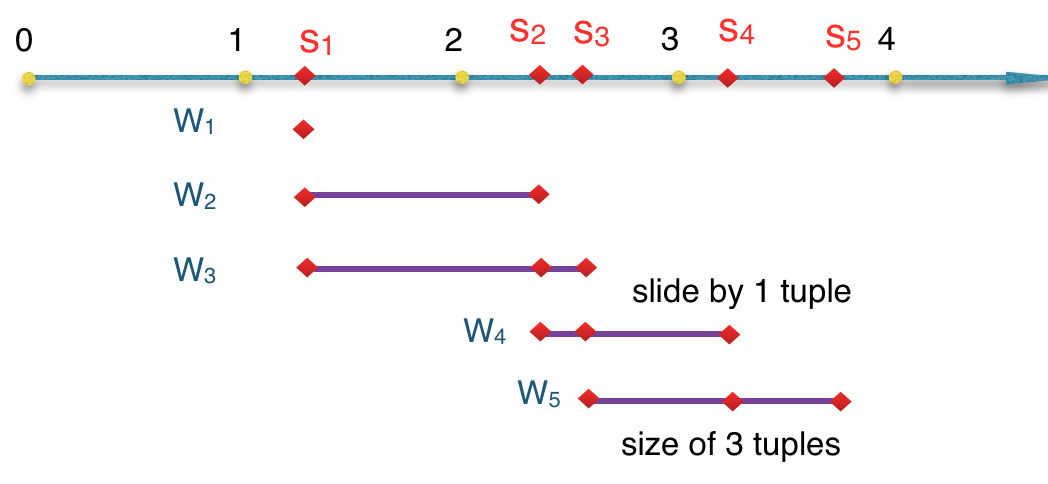
\includegraphics[width=0.7\textwidth]{slideWin}
\caption{Sliding Window}
\label{fig:slideWin}
\end{figure}


\item \textbf{Tumbling window}: a particular sliding window where the boundaries move is equal to the window's width. Windows are disjoint or non-overlapped each other. However, windowed stream will still cover all elements on based stream.

For example, window contains last 2 transactions once every 2 transactions passed. Up to 5 a.m, the stream contains 3 windows (Figure~\ref{fig:tumblingWin})

\begin{itemize}
\item $W_1:\{s_1,s_2\}$ 
\item $W_2:\{s_3, s_4\}$ 
\item $W_3:\{s_5,s_6\}$ 
\end{itemize}

\begin{figure}[htbp!] 
\centering    
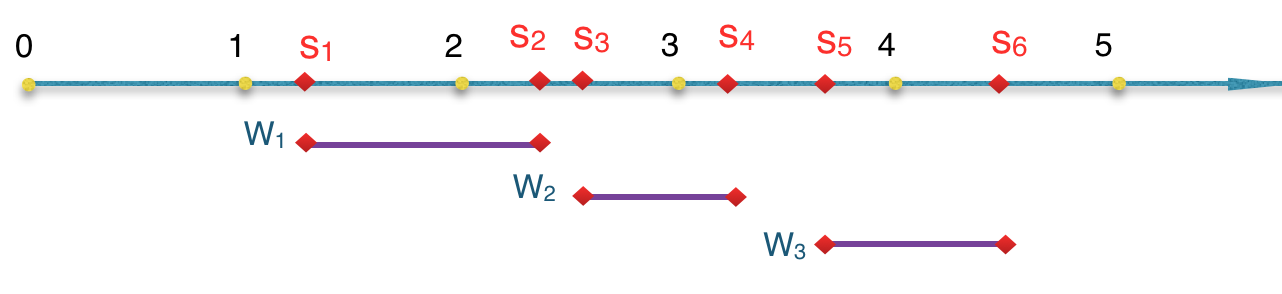
\includegraphics[width=0.8\textwidth]{tumblingWin}
\caption{Tumbling Window}
\label{fig:tumblingWin}
\end{figure}


\item \textbf{Jumping window}: a particular sliding window where the boundaries move is larger than the window's width. Windows are disjoint or non-overlapped each other but some of tuples may be discarded. For example, window contains last 2 transactions once every 4 transactions passed. Up to 5am, the stream contains 2 windows (Figure~\ref{fig:jumpingWin})
\begin{itemize}
\item $W_1:\{s_3,s_4\}$ when $s_4$ has arrived, window buffer contains 4 tuples $\{s_1,s_2,s_3,s_4\}$ but window's width is 2 so that $\{s_1,s_2\}$ will be evicted from window. Window buffer keeps $\{s_3,s_4\}$ then emits buffer as window $W_1$.
\item $W_2:\{s_7, s_8\}$ window buffer evicts $\{s_5,s_6\}$, keeps $\{s_7,s_8\}$ then emits buffer as window $W_2$.
\end{itemize}

\begin{figure}[htbp!] 
\centering    
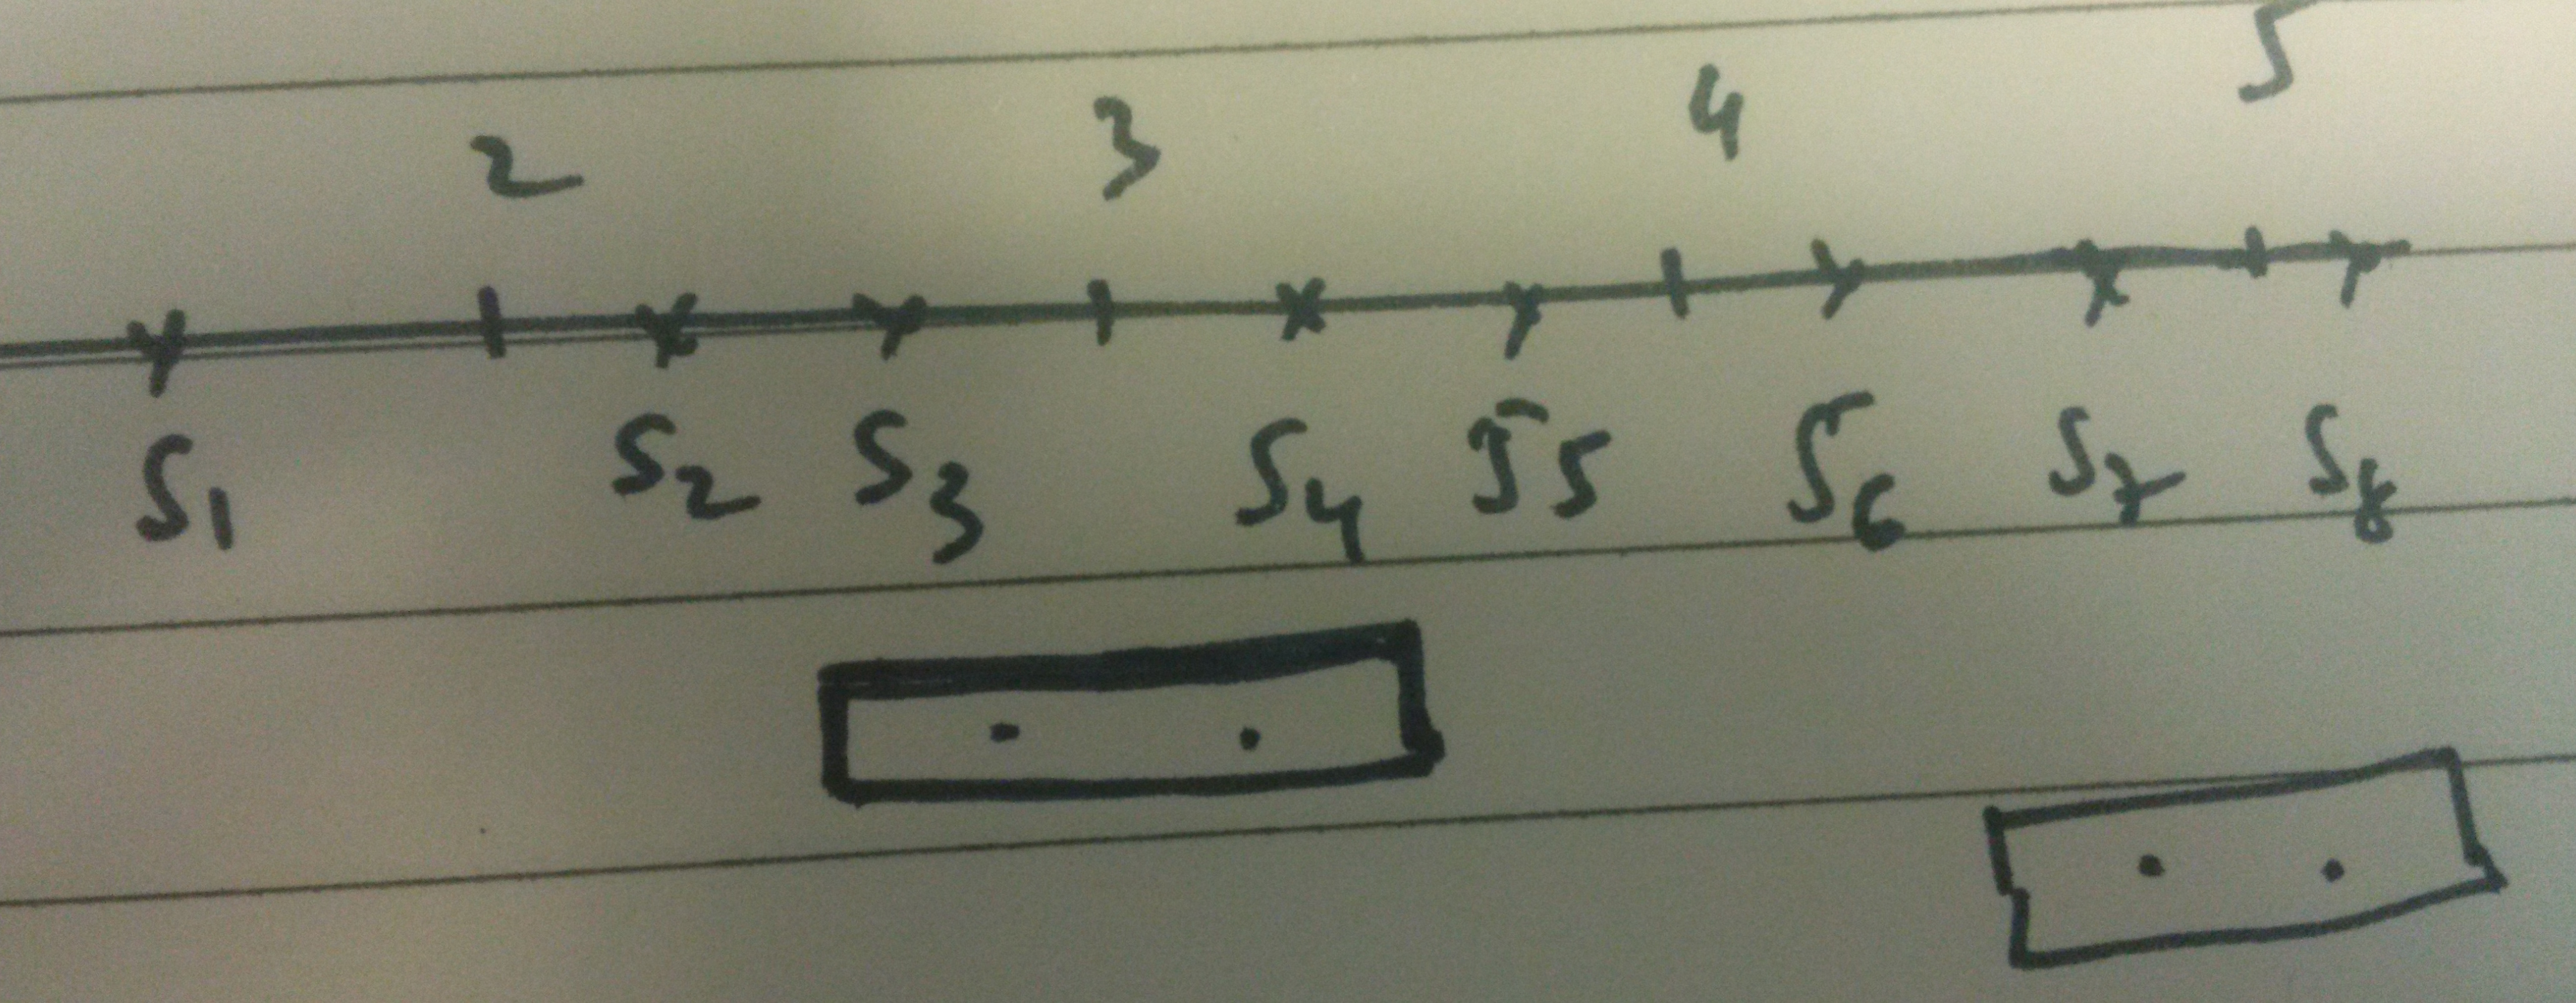
\includegraphics[width=1\textwidth]{jumpingWin}
\caption{Jumping Window}
\label{fig:jumpingWin}
\end{figure}


\end{itemize}


\subsection{Definition of contents} 

\begin{itemize}
	\item \textbf{Logical} or t\textbf{ime-based windows} are defined in terms of time interval, e.g., a time-base sliding window may maintain the the last one minute of data.
	
	\item \textbf{Physical} (also known as \textbf{count-based} or \textbf{tuple-based}) \textbf{windows} are defined in terms of the number of tuples, e.g., a count-based window may store the last arrived 100 tuples.
	
	\item \textbf{Delta-based windows} are defined in terms of a delta function and a threshold value. The function calculates a delta between 2 elements such as absolute distance or Euclidean distance between them. In delta-based windows, the delta between the first element and any of the rest must not be larger than the threshold, respectively. Currently new arrival data point will join the window if the delta between it and the first elements of window is equal or less than threshold. Otherwise, the window is closed and emitted; the currently arrival data point trigger a new window. 
	
Formally, a delta windows $W$ contains $n$ interval ordered elements $s_1, s_2,...,s_n$ continuously so that every elements $a_k$ with $k \in [1,n]$ must satisfies
	\begin{equation}
		\Delta(s_1,s_k) \leq \phi
	\end{equation}

There is a new arrival tuple $s_{n+1}$.
\begin{itemize}
\item if $\Delta(s_1,s_{n+1}) \leq \phi$, $s_{n+1}$ will join window $W$
\item Otherwise, window $W$ is closed and emitted for further computation. $s_{n+1}$ will trigger new window $W': \{s_{n+1}\}$
\end{itemize}

	
For example, assuming that stream $S$ contains 4 tuples so far (Figure~\ref{fig:deltaWin}). Element in window $W$ must satisfy the condition that the absolute distance between it and the first elements is not higher than 10.

Up to the moment $s_4$ has processed, Stream $S$ is discretized into window streams of 
\begin{itemize}
\item $W_1:\{s_1,s_2, s_3\}$ satisfies $\Delta(s_k,s_1) =|s_k-s_1| < 10 $ where $k \in [1,3]$
\item $W_2:\{s_4\}$ because $\Delta(s_4,s_1) = |s_4-s_1| = 12 > 10$, $s_4$ trigger a new window $W_2$
\end{itemize}

\begin{figure}[htbp!] 
\centering    
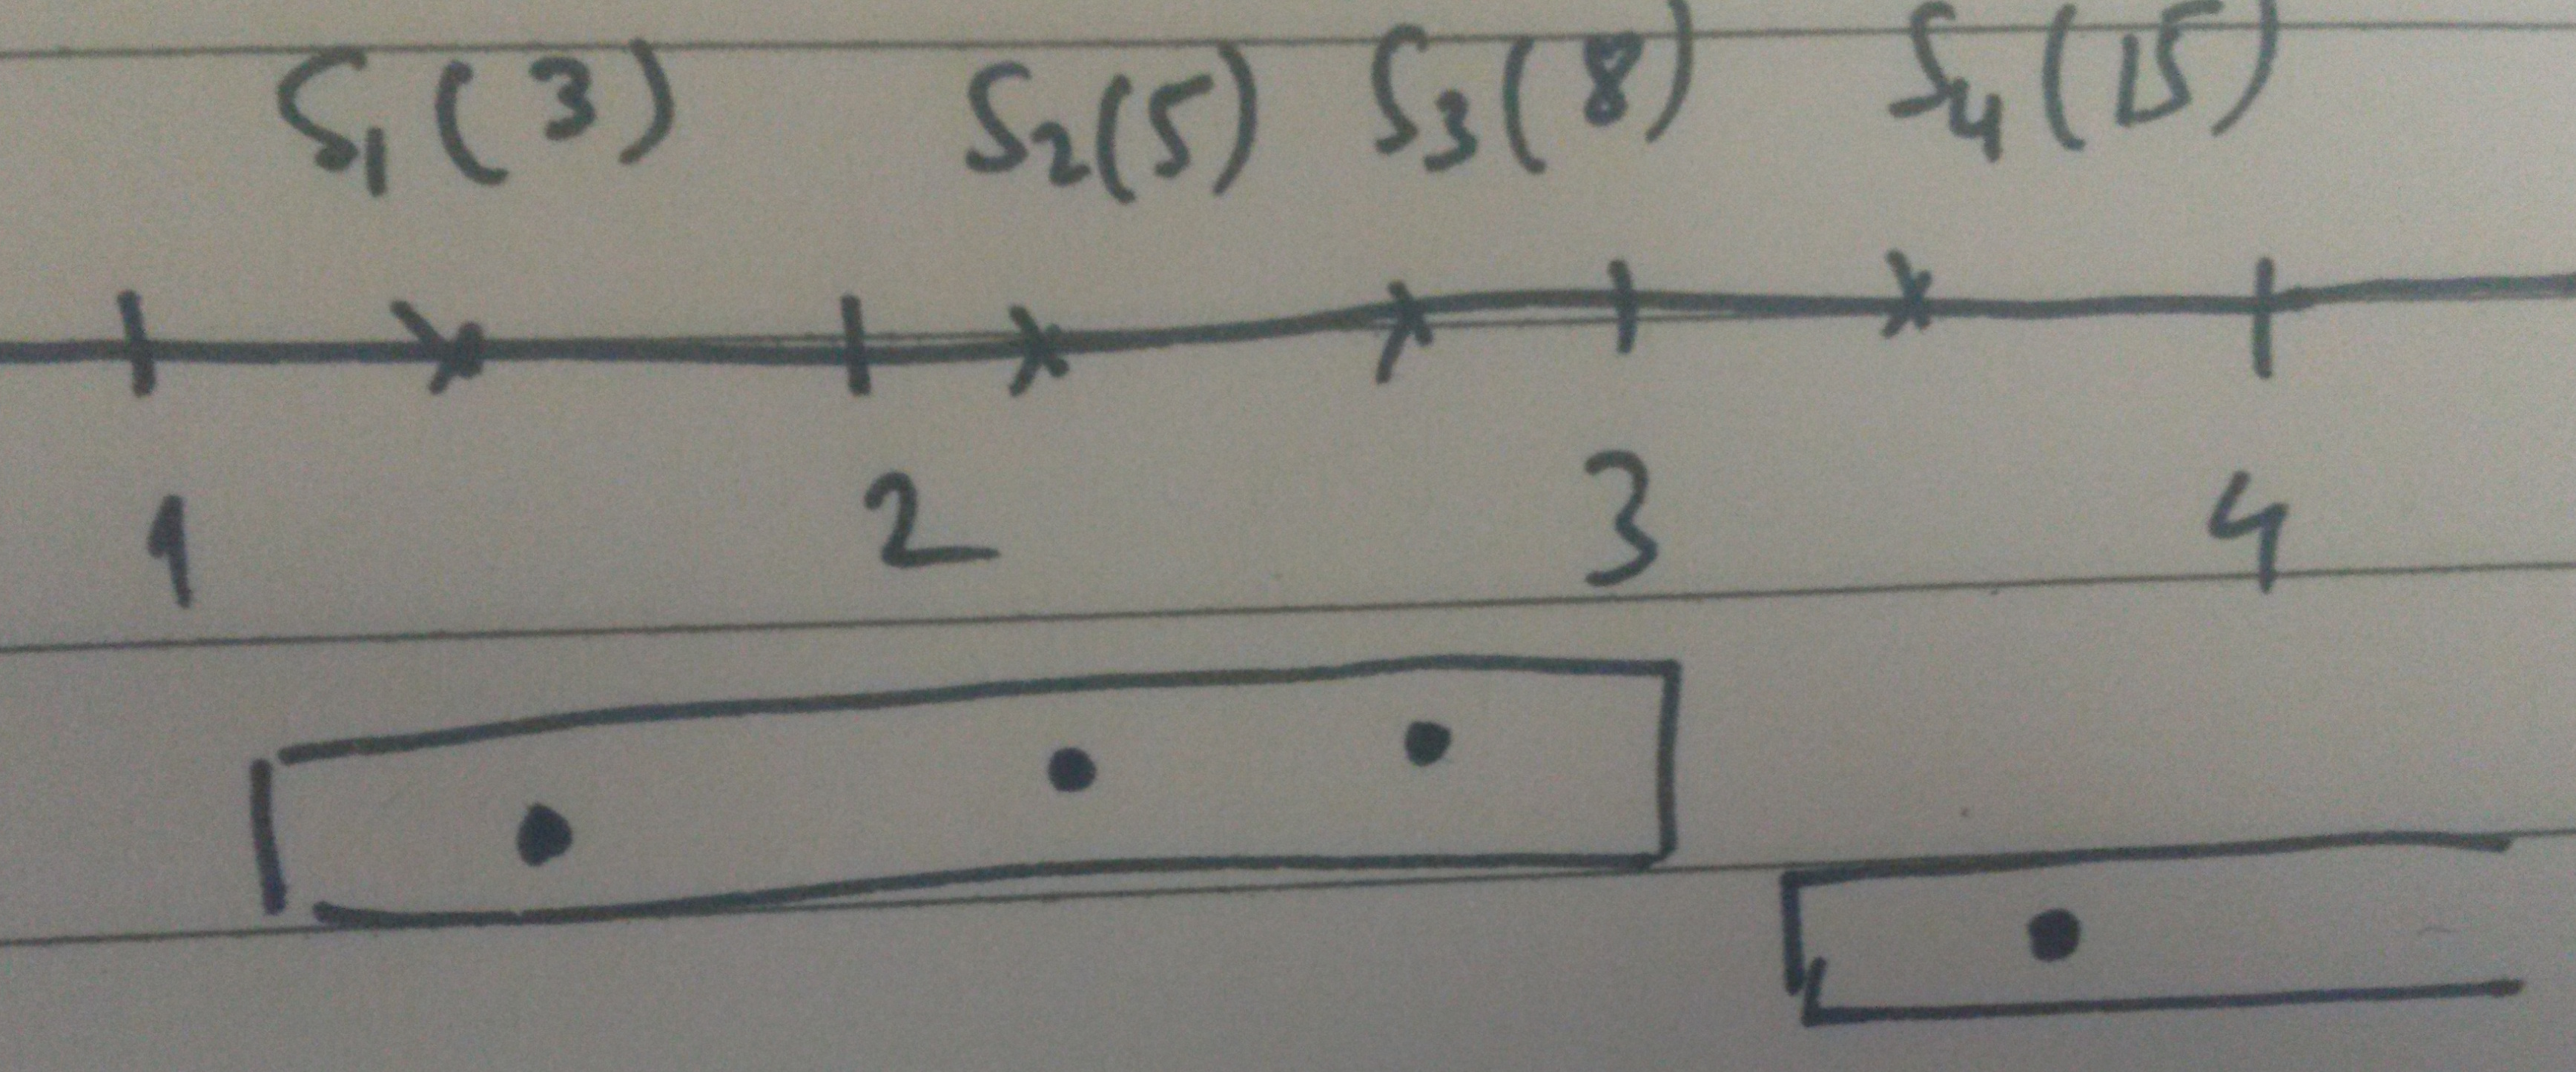
\includegraphics[width=1\textwidth]{deltaWin}
\caption{Delta-based Window}
\label{fig:deltaWin}
\end{figure}



	\item \textbf{Partitioned windows} contain only the elements  in the same group which differentiates itself from the other groups  by the value of a grouping attributes (subset of its schema), e.g., a partitioned window store last 100 elements with the same value of (\textit{StockSymbol}, \textit{Exchange})(Figure~\ref{fig:partitionedWin}). Thus, several substreams are derived logically from the base stream, each one is represented by an existing combinations of value $<a_1,a_2,...,a_k> \in Dom(S)$ on the grouping attributes $<A_1, A_2,...,A_k> \subset S$ ($S$ is schema of tuples, $Dom(S)$ is domain of $S$). Each group maintains a separate window buffer to capture arrival events and emit or apply Opertors on the buffer when appropriate.
	
\begin{figure}[htbp!] 
\centering    
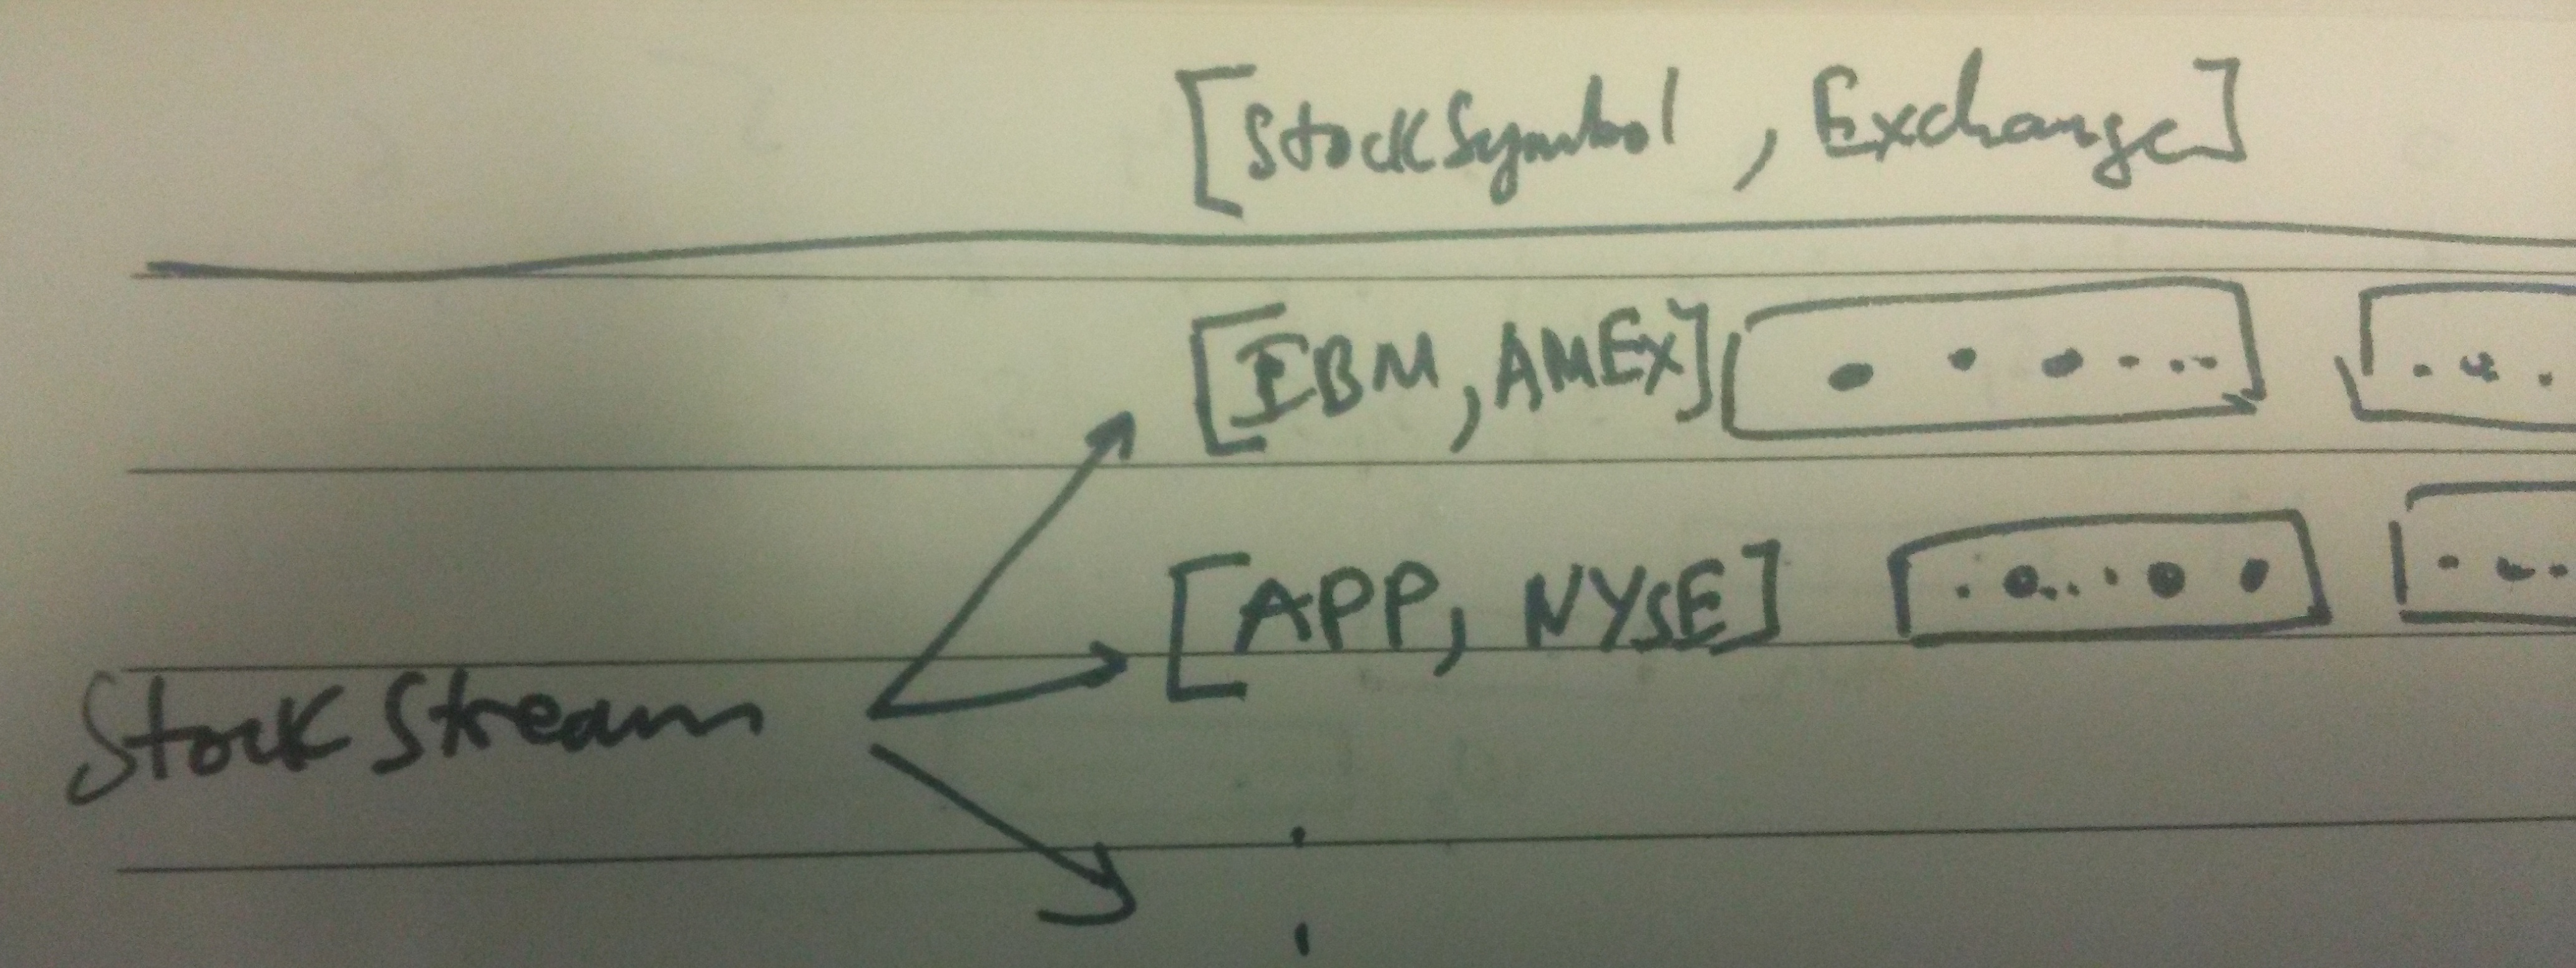
\includegraphics[width=1\textwidth]{partitionedWin}
\caption{Partitioned Window}
\label{fig:partitionedWin}
\end{figure}
	
%	\textbf{TODO: check Towards a Streaming SQL standard page 1385}
	
	
	
	\item \textbf{Predicate windows}~\citep{Ghanem:2008}, in which an arbitrary logical predicate specifies the contents. Only tuples that satisfies the predicate will join the window, otherwise it is discarded e.g.,predicate window maintains last 100 transactions which have more than 100.000 units in terms of \textit{volume}, respectively. Every transaction with fewer quantity will be discarded.
	
\end{itemize}

%\subsection{Frequency of movement[Optional]} jumping window, mixed jumping window, tumbling window

%By default, a time-based window is updated at every time tick, and a count-based window is updated when a new tuple arrives. A jumping window is updated every k ticks or after every kth arrival. Note that a count-based window may be updated periodically, and a time-based window may be updated after some number of new tuples have arrived; these are referred to as mixed jumping windows [Ma et al., 2005]. If k is equal to the window size, then the result is a series of non-overlapping tumbling windows [Abadi et al., 2003].
%In practice, tumbling windows, such as the one-minute windows in query Q1 from Sec- tion 2.1.1, are popular due to the simplicity of their implementation—at the end of each window, the query resets its state and starts over. Forward-sliding windows (time-based and count-based) are also appealing due to their intuitive semantics, especially with joins and aggregation, as we will discuss below. However, sliding windows are more difficult to implement than tumbling windows; over time, a continuous query must insert new tuples into a window and remove expired tuples that have fallen out of the window range.


%\textbf{//TODO}:(check Sliding Window Query Processing over Data Stream pages 25)


%The notion of sliding windows requires at least an ordering on data stream elements. In many cases, the arrival orders of the elements suffices as an \"implicit timestamp\" attached to each data element. However, sometimes it is preferable to user \"explicit timestamp\" provided as part of data stream. Formally, we say that a data stream consists of a set of (tuple, timestamp) pairs. Timestamp attribute could be a traditional timestamp or it could be a sequence number - all that is required is that it come from a totally ordered domain with a distance metric. The ordering induced by the timestamp is used when selecting the data elements making up a sliding window. 


%\textbf{Notes}: in CQL tuple-based sliding window may be non-deterministic - and therefore may not be appropriate - when timestamp are not unique


%\textbf{Notes}: Tuple relational calculus by Edgar F. Codd

%\textbf{Notes}: \href{http://en.wikipedia.org/wiki/Relational\_algebra}{http://en.wikipedia.org/wiki/Relational\_algebra}

